The next model we consider is an agent-based model. Each individual in the population can be in either of 7 states discussed above: susceptible, exposed, infected, hospitalized, funeral, recovered or dead. The flow between two states is a  probability of transition from one state to another for a typical individual. We represent our model in Figure~\ref{ABM}. In each time step a typical individual who is susceptible to contracting a virus can either transition to exposed state with probability $p_{SE}$ or stay susceptible with probability $p_{SS}$. An individual in the exposed state transitions to infected with probability $p_{EI}$ and stays exposed with probability $p_{EE}$. An individual who is infected can stay infected, recover, go to a hospital or die and transition to funeral state with probabilities $p_{II},\, p_{IR},\, p_{IH}$ and $p_{IF}$ respectively. Recovery is considered a terminal state so individuals in this state stay in it for the remaining duration of the simulation. Hospitalized individuals may stay hospitalized, transition to recovered or funeral with probabilities $p_{HH}, \, p_{HR}$ and $p_{HF}$. We assume that the individual who dies from Ebola remains infectious through the duration of the entire burial ceremony and no precautions are taken against disease transmission. Safely buried individuals are considered dead and noninfectious and remain in this state for the remaining time of the simulation.  

%  \begin{tikzpicture}[node distance=2cm, font=\tiny]
%        \node [draw, terminal]  (start) at (0,0) {Start};
%        \node [draw, predproc, right of= start] (acquire)(write) {Acquire Image};
%
%%% paths
%    \draw[->](work) -- node[above]{yes}(end);
%    \end{tikzpicture}
\begin{figure}[h!]
\begin{center}
\begin{tikzpicture}[->,>=stealth',shorten >=1pt,auto,node distance=3cm,
  thick,main node/.style={circle,fill=blue!20,draw,font=\sffamily\Large\bfseries}]

  \node[main node] (1) {S};
  \node[main node] (2) [right of=1] {E};
  \node[main node] (3) [right of=2] {I};
  \node[main node] (4) [right of=3] {R};
    \node[main node] (5) [below left of=3] {D};
      \node[main node] (6) [below right of=3] {F};
        \node[main node] (7) [right of=6] {H};

  \path[every node/.style={font=\sffamily\small}]
    (1)
        edge node {$p_{SE}$} (2)
        edge [loop above] node {$p_{SS}$} (1)
    (2) 
        edge node {$p_{EI}$} (3)
         edge [loop above] node {$p_{EE}$} (2)
      
    (3) 
       edge node {$p_{IR}$} (4)
       edge node[left] {$p_{IF}$} (6)
       edge node {$p_{IH}$} (7)
        edge [loop above] node {$p_{II}$} (3)
    (4)
         edge [loop above] node {$p_{RR}$} (4)
       
(6) edge node{$p_{FD}$} (5) 
edge [loop below] node {$p_{FF}$} (6)     
(7) edge node[right]{$p_{HR}$} (4) 
edge [loop below] node {$p_{HH}$} (7)
  (7) edge node{$p_{HF}$} (6)      
 (5) edge [loop below] node {$p_{DD}$} (5)
        ;
        
\end{tikzpicture}
\end{center}
\caption{Spread of the disease: Agent-based model. Each node represents a typical individual's state. An individual can transition to a state to which he is connected by a directed arc with a probability specified on an arc.}
\label{ABM}
\end{figure}
Let

\begin{itemize}
\item[]$t_{IP}$ be the incubation period, i.e. time during which the individual has the virus in his body but does not yet show severe symptoms
\item[] $t_{ID}$ infection duration time after the onset of severe symptoms
\item[] $t_{H}$ time to hospitalization after manifestation of severe symptoms
\item[] $t_{IF}$ time from the onset of severe symptoms to funeral
\item[] $t_{HF}$ time from patient's arrival at the hospital to funeral
\item[] $t_{HR}$ time from patient's arrival at the hospital to recovery
\item[] $t_{DF}$ duration of traditional funeral
\item[] $N$  total number of individuals in a population
\item[] $N_{I}$  total number of individuals in the infected state
\item[] $N_{H}$  total number of individuals in the hospitalized state
\item[] $N_{F}$  total number of individuals in the funeral state
\item[] $\beta_{I}$ rate at which the disease spreads during an interaction with an infected person
\item[] $\beta_{H}$ rate at which the disease spreads during an interaction with a hospitalized person
\item[] $\beta_{F}$ rate at which the disease spreads during an interaction with a person who is in the funeral state
\end{itemize}
We define the individual's probability of transition for each state as

\begin{subequations}
\begin{alignat}{1}
&p_{SE}=\beta_I\cdot \frac{N_{I}}{N}+\beta_H\cdot \frac{N_{H}}{N}+\beta_F\cdot\frac{ N_F}{N}\\
&p_{SS}=1-p_{SE}\\
&p_{EE}=1-\frac{1}{t_{IP}}\\
&p_{EI}=\frac{1}{t_{IP}}\\
&p_{II}=\frac{1}{t_{ID}}\\
&p_{IH}=\frac{1}{t_{H}}\\
&p_{IF}= \frac{1}{t_{IF}}\\
&p_{IR}=1-p_{II}-p_{IH}-p_{IF}\\
&p_{HF}=\frac{1}{t_{HF}}\\
&p_{HR}=\frac{1}{t_{HR}}\\
&p_{HH}=1-p_{HF}-p_{HR}\\
&p_{FF}=\frac{1}{t_{DF}}\\
&p_{FD}=1-p_{FF}\\
&p_{RR}=1\\
&p_{DD}=1
\end{alignat}
\end{subequations}
\subsection{Simulation}
We consider a population of size 1000 with 999 individuals starting in a susceptible state and 1 individual in the exposed state. Numeric probabilities of an individual transitioning from each state are recorded in Table~\ref{tab:probabilities}. We repeat the process 100 times and record the average outcome.  
Since are model is not deterministic, each time we would see different final outcome. Interestingly, there are basically only two different scenarios. There could be no outbreaks of Ebola but a severe spread of the disease could also happen. During the 100 simulations, 27 of them show no outbreak of Ebola, which means less then 1\% of people get the disease. But on the other hand, 73 experiments show that there will be severe outbreak of disease, more than 90\% of people would get infected. A histogram for simulation outcomes is depicted in Figure~\ref{fig:Hist}.
%
%
% HERE IS THE PROBABILITY TRANSITION TABLE
%
%
%
%
\begin{table}[h!]
\caption{Agent-Model Parameters for Ebola Epidemic in Liberia Before and After the International Intervention} % title of Table
\centering % used for centering table
\begin{tabular}{c c c } 
\hline\hline %inserts double horizontal lines
Parameter & Liberia Before Intervention  & Liberia After Intervention \\ [0.5ex] 
 & (Mar/14 to Sept/14) &  (Sept/14 to Jul/15) \\ [0.5ex] % inserts table
% inserts table
%heading
\hline % inserts single horizontal line
$p_{SE}$ & \textbf{DYNAMIC} & \textbf{DYNAMIC} \\ 
$p_{SS}$ & \textbf{COMPUTE}8 & \textbf{COMPUTE}  \\ 
$p_{EE}$ & 0.9091 & 0.9091  \\ 
$p_{EI}$ & 0.0909 & 0.0909  \\ 
$p_{II}$ & 0.1 & 0.1  \\ 
$p_{IH}$ & 0.2227 & 0.2160  \\ 
$p_{IF}$ & 0.125 & 0.125  \\ 
$p_{IR}$ & 0.5523 & 0.559  \\ 
$p_{HF}$ & 0.2849 & 0.2849 \\ 
$p_{HR}$ & 0.1815 & 0.1815 \\ 
$p_{HH}$ & 0.5336& 0.5336  \\ 
$p_{FF}$ & 0.5 & 0.5 \\ 
$p_{FD}$ & 0.5 & 0.5  \\ 
$p_{RR}$ & 1 & 1  \\ 
$p_{DD}$ & 1 & 1 \\ [1ex] 
\hline 
\end{tabular}
\label{tab:probabilities}
\end{table}

\begin{figure}
\begin{center}
\includegraphics[scale=0.5]{N1000Hist.eps}
\end{center}
\caption{Histogram showing the outcome of 100 simulations.}
\label{fig:Hist}
\end{figure}


%%%%%%%%%%%%%%%%%%%%%%%%%%%%%%%%%%%%
% figure N1000Hist.eps
%%%%%%%%%%%%%%%%%%%%%%%%%%%%%%%%%%%%
In our agent based model, all the simulations reach their final stationary states before $t = 500$. We plot the final results of 100 simulations in one graph. There many cases we don't observe any severe outbreak of Ebola. However there are many cases which show catastrophic disease. If the disastrous disease happens, on average, 95\% of people would get the disease and 76\% of people would die from it, as presented in Figure~\ref{fig:Scatter100}. 

%%%%%%%%%%%%%%%%%%%%%%%%%%%%%%%%%%%%
% figure N1000Scatter.eps
%%%%%%%%%%%%%%%%%%%%%%%%%%%%%%%%%%%%
 
\begin{figure}
\begin{center}
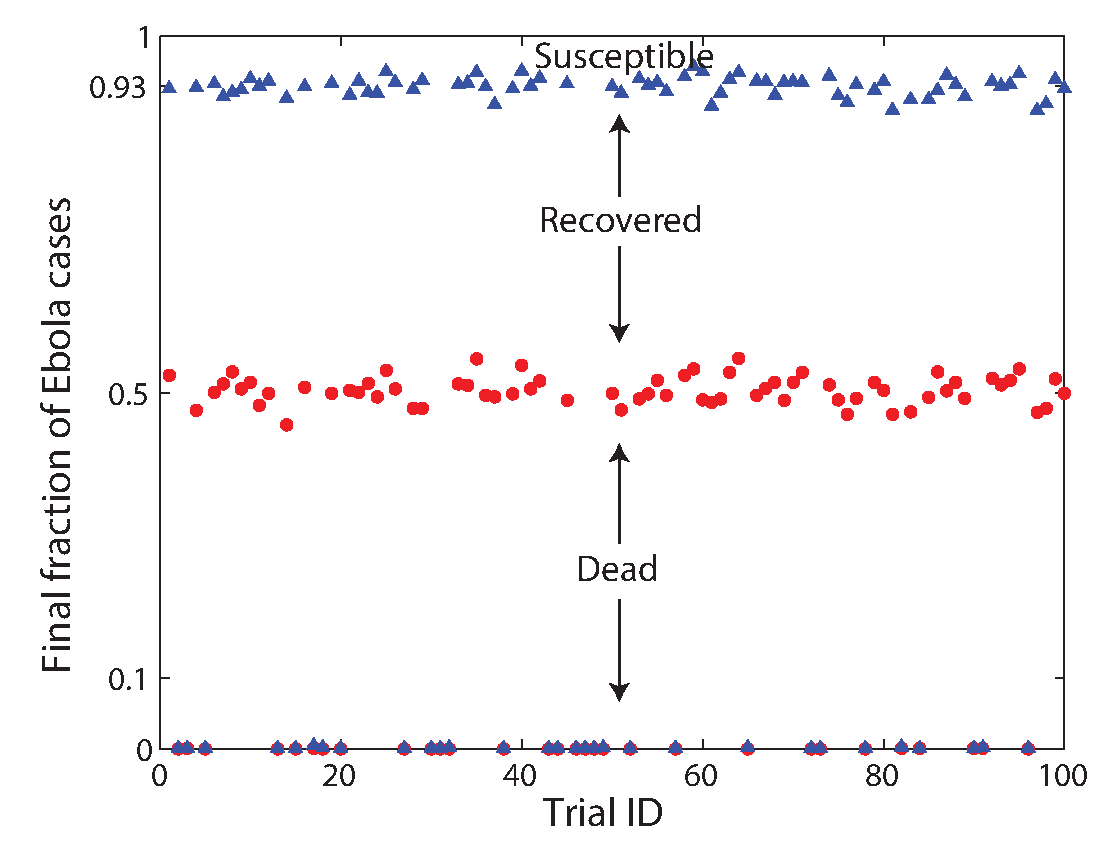
\includegraphics[scale=0.5]{N1000Scatter.eps}
\end{center}
\caption{Scatter plot showing the proportion of population that contracts a disease and the proportion of the population that dies due to the disease for a population size 1000}
\label{fig:Scatter}
\end{figure}

%%%%%%%%%%%%%%%%%%%%%%%%%%%%%%%%%%%%
% figure N1000Scatter.eps
%%%%%%%%%%%%%%%%%%%%%%%%%%%%%%%%%%%%

If there is no outbreak, the infected agent may or may not infect some agent in the system, but the majority of people stay susceptible. The infected agents will recover or die before they can infect more people. The amount of people getting Ebola is relatively very low, so all seven states stay mostly like constant all the time. Illustration of this case is presented in Figure~\ref{fig:NoOutbreak}.
\begin{figure}
\begin{center}
\includegraphics[scale=0.8]{NoOutbreak.eps}
\end{center}
\caption{No outbreak realization of the outbreak process}
\label{fig:NoOutbreak}
\end{figure}

%%%%%%%%%%%%%%%%%%%%%%%%%%%%%%%%%%%%
% figure NoOutbreak.eps
%%%%%%%%%%%%%%%%%%%%%%%%%%%%%%%%%%%%

On the other hand, if the infected agent contacts many people during the states infected (I), hospitalized (H), or funeral (F) before he or she dies or recovers, then there would be a disastrous outbreak of disease, as shown in Figure~\ref{fig:Outbreak}. People getting the disease would grow exponentially until $t = 125$. That is also the time people in I, H, and F reach their peaks. After this time, the system doesn't have enough susceptible agents to spread the disease, so the increasing rate of people getting Ebola starts slowing down, and the amount of agents in I, H, and F start decreasing too. Around $t = 180$ I, H, and F reach zero, S stops growing, no more new agents get Ebola. That means the dynamic stops, the system reaches its stationary state. All the agent at this time would either be in S, R or D. These are the recurrent states in this Markov chain, and all other four states are transient states. As we showed before, on average, 5\% of people would stay in state S, 19\% of people stay in R, and 76\% of people stay in D. 
%%%%%%%%%%%%%%%%%%%%%%%%%%%%%%%%%%%%
% figure Outbreak.eps
%%%%%%%%%%%%%%%%%%%%%%%%%%%%%%%%%%%%
\begin{figure}
\begin{center}
\includegraphics[scale=0.8]{Outbreak.eps}
\end{center}
\caption{Realization in which outbreak occurs}
\label{fig:Outbreak}
\end{figure}

%%%%%%%%%%%%%%%%%%%%%%%%%%%%%%%%%%%%
% figure Outbreak.eps
%%%%%%%%%%%%%%%%%%%%%%%%%%%%%%%%%%%%



As the system evolves, we can plot the states we are interested in the most in a phase portrait. We keep track of amount of agents who don't get the disease and the amount of people who die from the disease or recover from it and present a phase portrait in Figure~\ref{fig:PhasePortraitABM}. We put the ratio of S to the total population on the x-axis, and put the ratio of D plus R to the total population on the y-axis. Each time we plot the these three quantities as a dot in the 2-D box. When $t = 0$, we have one agent in state E, which means 99.9\% of agents are in state S, and all other states contain no agents. If no severe outbreak happen, the system would stay stable, only negligible amount of people get Ebola, the dot would remain basically the same position as time goes by. However, if there is an outbreak, the trajectory would gradually move to its final state, on average, it would be $(S, [R]+[D]) = (0.05, 0.95)$. We can see the it would be a concave up function. We plot ten experiments and see their trajectories at the same time. Since the total sum of people in ration is one, all the final states in different experiments would go to points on the $x + y = 1$ line. The system starts at $(S, [R]+[D]) = (0.999, 0)$, a point very close to this line. If we see an outbreak, before the system reaches its final state, the distance of this point at any time $t$ would be the amount of agencies in the transient states E, I, H and F. But finally when the system stops evolving, we will see the dot goes to a point on this  $x + y = 1$ line. 

%%%%%%%%%%%%%%%%%%%%%%%%%%%%%%%%%%%%
% figure PhasePortrait.eps
%%%%%%%%%%%%%%%%%%%%%%%%%%%%%%%%%%%%
\begin{figure}[h!]
\begin{center}
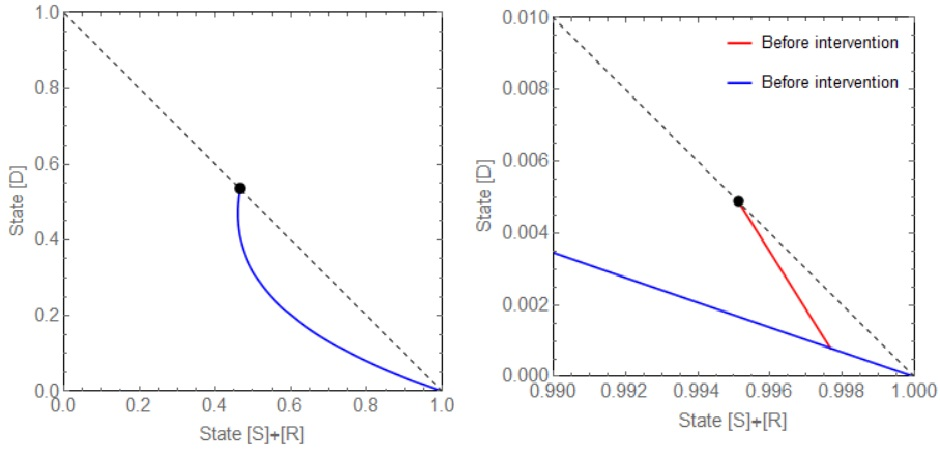
\includegraphics[scale=0.5]{PhasePortrait.eps}
\end{center}
\caption{Phase portrait: proportion of the population who are in susceptible state vs. population of the population who contracted Ebola for different uncertainty realizations.}
\label{fig:PhasePortraitABM}
\end{figure}

%%%%%%%%%%%%%%%%%%%%%%%%%%%%%%%%%%%%
% figure PhasePortrait.eps
%%%%%%%%%%%%%%%%%%%%%%%%%%%%%%%%%%%%

As in the system dynamic approach, we perform an intervention in our agent-based system too. Since the scale of the two systems are not the same, we start our intervention at a different time to the one in system dynamic approach. If we see an outbreak, we will intervene the system when 1\% of people get the disease. When the intervention starts, we change our three $\beta$, the contact rates of different ways people can get Ebola, which change the behavior of agents the most. Our results, presented in Figure~\ref{fig:Intervention}, show that if we start the intervention at 1\% of people get Ebola, finally 4\% of agents would get the disease, 1\% of agents would recover, and 3\% of agents would die. We wouldn't see a disastrous outbreak of disease comparing to the case without intervention. 

%%%%%%%%%%%%%%%%%%%%%%%%%%%%%%%%%%%%
% figure InterventionZoomIn.eps
%%%%%%%%%%%%%%%%%%%%%%%%%%%%%%%%%%%%

\begin{figure}[h!]
\begin{center}
\includegraphics[scale=0.8]{InterventionZoomIn.eps}
\end{center}
\caption{Effect of Intervention on the spread of the disease }
\label{fig:Intervention}
\end{figure}

%%%%%%%%%%%%%%%%%%%%%%%%%%%%%%%%%%%%
% figure InterventionZoomIn.eps
%%%%%%%%%%%%%%%%%%%%%%%%%%%%%%%%%%%%

We can try our agent based model on different scales. Aside from $N = 1000$ we did before, set the total population to be $N = 100$ and $5000,$ we can see how the size of population affects the spread of disease. The results are presented in Figure~\ref{fig:VarPopSize}. As we can see in the following figures, when we increase the population size, although the average of final S, D, and R states stay the same, the standard deviations of these quantities are smaller larger systems. The bands of people who get Ebola and die would become narrower as we increase the population size. Hence we might suggest that the system become more stable, and the final results are more predictable for larger systems.

%%%%%%%%%%%%%%%%%%%%%%%%%%%%%%%%%%%%
% figure N100Scatter.eps, N5000Scatter.eps
%%%%%%%%%%%%%%%%%%%%%%%%%%%%%%%%%%%%

\begin{figure}[h!]
 \centering 
 \begin{subfigure}[b]{0.45\textwidth}
  \includegraphics[width=\textwidth]{N100Scatter.eps} \caption{Scatter plot showing the proportion of population that contracts a disease and the proportion of the population that dies due to the disease for a population size 100.} \label{fig:Scatter100} \end{subfigure}
 %
 \hspace{.1cm}
\begin{subfigure}[b]{0.45\textwidth}
 \includegraphics[width=\textwidth]{N5000Scatter.eps} \caption{Scatter plot showing the proportion of population that contracts a disease and the proportion of the population that dies due to the disease for a population size 5000.} \label{fig:Scatter5000} \end{subfigure} \caption{Effect of changing the population size on the proportion of the diseased population}
\label{fig:VarPopSize} 
\end{figure}

%%%%%%%%%%%%%%%%%%%%%%%%%%%%%%%%%%%%
% figure N100Scatter.eps, N5000Scatter.eps
%%%%%%%%%%%%%%%%%%%%%%%%%%%%%%%%%%%%




%%%%%%%%%%%%%%%%%%%%%%%%%%%%%%%%%%%%
%%%%%%%%%%%%%%%%%%%%%%%%%%%%%%%%%%%%
%%%%%%%%%%%%%%%%%%%%%%%%%%%%%%%%%%%%









